
          %-------------------------------%
\chapter{~~Finite elements and integrators}\label{\numb section 6}
          %-------------------------------%


Finite elments are still incipient in \maniFEM.
Paragraph \ref{\numb section 6.\numb parag 1} discusses the concept of finite element
and paragraphs \ref{\numb section 6.\numb parag 2} -- \ref{\numb section 6.\numb parag 10}
give examples of use.
There is a lot of ongoing work on this subject.

{\ManiFEM} distinguishes between cells (which are geometric entities) and finite elements.
We may have different finite elements whose geometry is the same.
For instance, we may have triangular Lagrange finite elemens of different degrees;
they will all {\small\tt dock\_\,on} the same triangular cell.
See e.g.\ paragraph \ref{\numb section 6.\numb parag 5}.

Finite elements in {\maniFEM} can be divided in two categories.
Finite elements based on symbolic computations, using Gauss quadrature on a master element,
are discussed in
paragraphs \ref{\numb section 6.\numb parag 2} -- \ref{\numb section 6.\numb parag 8}.
They are flexible (we can compute integrals of arbitrary expressions) but quite slow
(because they rely strongly on symbolic manipulation of expressions).
They can be interesting for dydactic purposes.%
\footnote{They are also very useful for validating other types of finite elements.}
Finite elements described in paragraphs \ref{\numb section 6.\numb parag 9} and
\ref{\numb section 6.\numb parag 10} are much faster at the cost of a tedious internal
implementation.
Also, from the point of view of the final user, their syntax is slightly less elegant.


          %---------------%
\section{~~Finite elements}\label{\numb section 6.\numb parag 1}
          %---------------%

The notion of finite element is quite complex.
The purpose of a {\small\tt\verm{FiniteElement}} is to build a list of functions, say, $ \psi $,
defined on our mesh.
The linear span of these functions will be a finite-dimensional Hilbert space
(the discretization of an infinite-dimensional Sobolev space).
It is the {\small\tt\verm{FiniteElement}}'s job to replace, in the variational formulation,
the unknown function by one $ \psi $, the test function by another $ \psi $ and,
by evaluating the integrals, obtain the coefficients of a system of linear equations.
Some external solver will then solve the system, and it is the job of the finite element
to transform back the vector produced by the solver into a function defined on our mesh.

Computing each integral is a somewhat separate process; it's the job of an
{\small\tt\verm{Integrator}}
which could be a Gauss quadrature or some other procedure like symbolic integration.
The separation between a {\small\tt\verm{FiniteElement}}'s job and
the {\small\tt\verm{Itegrator}}'s job is not very sharp.
For instance, the Gauss quadrature is often perfomed not on the physical cell but rather
on a master element which is built and handled by the {\small\tt\verm{FiniteElement}}.
The authors of {\maniFEM} have tried to separate these two concepts
as much as possible, especially because we may want to use a {\small\tt\verm{FiniteElement}}
with no master element, or an {\small\tt\verm{Integrator}} acting directly on the physical cell.

An object belonging to the {\small\tt class} {\small\tt\verm{FiniteElement}} is a mere wrapper
for a {\small\tt\verm{FiniteElement}::Core} (see paragraph \ref{\numb section 11.\numb parag 5}).
Several subclasses of {\small\tt\verm{FiniteElement}::Core} exist for different
kinds of finite elements.
There is a {\small\tt class} {\small\tt\verm{FiniteElement}::WithMaster} with subclasses like
{\small\tt\verm{FiniteElement}::} {\small\tt::WithMaster::Segment}, {\small\tt Triangle} and
{\small\tt Quadrangle}.
There is also a {\small\tt class} {\small\tt\verm{FiniteElement}::StandAlone} for elements
with no master, having its own subclasses for different geometries of the cell.

The final user does not need to worry about these details.
He or she will declare {\small\tt\verm{FiniteElement}}s (wrappers) of different types
by providing {\small\tt\textcolor{tag}{tag}}s to the constructor, as shown in
subsequent paragraphs of this section.

{\small\tt\verm{FiniteElement}}s with master keep as an attribute the map transforming
the master element to the current physical cell.
This map depends of course on the geometry of the cell and thus it must be computed from
scratch each time we begin integrating on a new cell.
We say that the {\small\tt\verm{FiniteElement}} is docked on a new {\small\tt\verm{Cell}};
the method {\small\tt dock\_\,on} performs this operation.
This method is element-specific, each type of finite element having its own class.

For instance, {\small\tt\verm{FiniteElement}}s declared with {\small\tt\textcolor{tag}{tag}%
::quadrangle} will only {\small\tt dock\_\,on} quadrilaterals
(two-dimensional {\small\tt\verm{Cell}}s with four sides).
% Recall that in {\maniFEM} the vertices do not have necessarily any number attached.
% When we create a {\small\tt\verm{FiniteElement}::Lagrange\_\,Q1} object, it will enumerate vertices
% of the mesh if a mesh exists already, and it will prepare the ground for vertices created
% in the future to be enumerated, too.
% This enumeration is useful to identify a vector of real numbers with the values
% (at each vertex) of a function defined on the mesh.
When docking on a cell, the {\small\tt\verm{FiniteElement}} object will build four
``shape functions'' and a transformation map (a diffeomorphism between a master element
occuppying the square $ [-1, 1]^2 $ and the current cell).
It will also build the jacobian of this transformation map (through symbolic differentiation).
The four shape functions can be accessed through the method {\small\tt basis\_\,function},
as shown in paragraph \ref{\numb section 6.\numb parag 2}.

It should be stressed that the approach presented in this section is rather low-level.
We are working hard to make {\maniFEM} understand statements describing variational
formulations given as {\tt C++} objects.
When this part of the code is done, the programming style will become much more elegant
and compact.

Note also that these examples make use of the {\small\tt Eigen} library.


          %------------------------------------------------%
\section{~~Laplace operator, Dirichlet boundary conditions}\label{\numb section 6.\numb parag 2}
          %------------------------------------------------%

Let's look at an example about the Laplace operator with non-homogeneous Dirichlet
boundary conditions.

\begin{Verbatim}[commandchars=\\\{\},formatcom=\small\tt,frame=single,
   label=parag-\ref{\numb section 6.\numb parag 2}.cpp,rulecolor=\color{coment},
   baselinestretch=0.94,framesep=2mm                                            ]
   \verm{Manifold} \azul{RR2} ( \textcolor{tag}{tag}::Euclid, \textcolor{tag}{tag}::of_dim, 2 );
   \verm{Function} \azul{xy} = RR2 .build_coordinate_system ( \textcolor{tag}{tag}::Lagrange, \textcolor{tag}{tag}::of_degree, 1 );
   \verm{Function} \azul{x} = xy [0], \azul{y} = xy [1];

   \cinza{// declare the type of finite element}
   \verm{FiniteElement} \azul{fe}
      ( \textcolor{tag}{tag}::with_master, \textcolor{tag}{tag}::quadrangle, \textcolor{tag}{tag}::Lagrange, \textcolor{tag}{tag}::of_degree, 1 );
   \verm{Integrator} \azul{integ} = fe .set_integrator ( \textcolor{tag}{tag}::Gauss, \textcolor{tag}{tag}::quad_4 );

   \cinza{// build a 10x12 mesh on a square domain}
   \verm{Cell} \azul{A} ( \textcolor{tag}{tag}::vertex );  x (A) = 0.;   y (A) = 0.;
   \verm{Cell} \azul{B} ( \textcolor{tag}{tag}::vertex );  x (B) = 1.;   y (B) = 0.;
   \verm{Cell} \azul{C} ( \textcolor{tag}{tag}::vertex );  x (C) = 1.;   y (C) = 1.;
   \verm{Cell} \azul{D} ( \textcolor{tag}{tag}::vertex );  x (D) = 0.;   y (D) = 1.;
   \verm{Mesh} \azul{AB} ( \textcolor{tag}{tag}::segment, A .reverse(), B, \textcolor{tag}{tag}::divided_in, 10 );
   \verm{Mesh} \azul{BC} ( \textcolor{tag}{tag}::segment, B .reverse(), C, \textcolor{tag}{tag}::divided_in, 12 );
   \verm{Mesh} \azul{CD} ( \textcolor{tag}{tag}::segment, C .reverse(), D, \textcolor{tag}{tag}::divided_in, 10 );
   \verm{Mesh} \azul{DA} ( \textcolor{tag}{tag}::segment, D .reverse(), A, \textcolor{tag}{tag}::divided_in, 12 );
   \verm{Mesh} \azul{ABCD} ( \textcolor{tag}{tag}::rectangle, AB, BC, CD, DA );
\end{Verbatim}

A finite element can handle by itself the numbering of vertices, as shown in paragraph
\ref{\numb section 6.\numb parag 4}.
For now, we prefer the conceptually simpler approach of building by hand a {\small\tt map}
for numbering vertices.

\begin{Verbatim}[commandchars=\\\{\},formatcom=\small\tt,frame=single,
   label=parag-\ref{\numb section 6.\numb parag 2}.cpp,rulecolor=\color{coment},
   baselinestretch=0.94,framesep=2mm                                            ]
   std::map < Cell, size_t > \azul{numbering};
   \verm{Mesh}::Iterator \azul{it} = ABCD .iterator ( \textcolor{tag}{tag}::over_vertices );
   size_t \azul{counter} = 0;
   for ( it .reset() ; it .in_range(); it++ )
   \{  \verm{Cell} \azul{V} = *it;  numbering [V] = counter;  ++counter;  \}
\end{Verbatim}

Paragraph \ref{\numb section 9.\numb parag 3} describe {\small\tt Iterator}s over
cells of a {\small\tt\verm{Mesh}}.

The matrix of the linear system and the vector holding the free coefficients
are declared as objects of the {\small\tt Eigen} library.

\begin{Verbatim}[commandchars=\\\{\},formatcom=\small\tt,frame=single,
   label=parag-\ref{\numb section 6.\numb parag 2}.cpp,rulecolor=\color{coment},
   baselinestretch=0.94,framesep=2mm                                            ]
   size_t \azul{size_matrix} = ABCD .number_of ( \textcolor{tag}{tag}::vertices );
   assert ( size_matrix == numbering .size() );
   Eigen::SparseMatrix < double > \azul{matrix_A} ( size_matrix, size_matrix );
   Eigen::VectorXd \azul{vector_b} ( size_matrix );  vector_b .setZero();
\end{Verbatim}

We now run over all rectangular cells of {\small\tt ABCD}, dock the finite element
on the current cell,
compute integrals of the form $ \displaystyle \int\!\!\!\int {\partial \psi_i \over
\partial x_\alpha} {\partial \psi_j \over \partial x_\beta} dx $ and add the obtained
values to the global matrix:

\begin{Verbatim}[commandchars=\\\{\},formatcom=\small\tt,frame=single,
   label=parag-\ref{\numb section 6.\numb parag 2}.cpp,rulecolor=\color{coment},
   baselinestretch=0.94,framesep=2mm                                            ]
   \cinza{// run over all square cells composing ABCD}
   \verm{Mesh}::Iterator \azul{it} = ABCD .iterator ( \textcolor{tag}{tag}::over_cells, \textcolor{tag}{tag}::of_max_dim );
   for ( it .reset(); it .in_range(); it++ )
   \{  \verm{Cell} \azul{small_square} = *it;
      fe .dock_on ( small_square );

      \cinza{// run twice over the four vertices of 'small_square'}
      \verm{Mesh}::Iterator \azul{it1} = small_square .boundary() .iterator ( \textcolor{tag}{tag}::over_vertices );
      \verm{Mesh}::Iterator \azul{it2} = small_square .boundary() .iterator ( \textcolor{tag}{tag}::over_vertices );
      for ( it1 .reset(); it1 .in_range(); it1++ )
      for ( it2 .reset(); it2 .in_range(); it2++ )
      \{  \verm{Cell} \azul{V} = *it1, \azul{W} = *it2;
         \cinza{// V may be the same as W, no problem about that}
         \verm{Function} \azul{psiV} = fe.basis_function(V),
                  \azul{psiW} = fe .basis_function (W),
                  \azul{d_psiV_dx} = psiV .deriv (x),
                  \azul{d_psiV_dy} = psiV .deriv (y),
                  \azul{d_psiW_dx} = psiW .deriv (x),
                  \azul{d_psiW_dy} = psiW .deriv (y);
                  
         \cinza{// 'fe' is already docked on 'small_square'}
         \cinza{// so this will be the domain of integration}
         matrix_A .coeffRef ( numbering[V], numbering[W] ) +=
            fe .integrate ( d_psiV_dx * d_psiW_dx + d_psiV_dy * d_psiW_dy );    \}  \}
\end{Verbatim}

In the above, {\small\tt coeffRef} is the method used by {\small\tt Eigen} to access elements of
a sparse matrix.

We impose Dirichlet boundary conditions $ u(x,y) = xy $ (this way, we know beforehand
the exact solution will be $ u(x,y) = xy $).
We use a function {\small\tt impose\_\,value\_\,of\_\,unknown} which changes the {\small\tt matrix\_\,A}
and the {\small\tt vector\_\,b} in order to impose the Dirichlet condition {\small\tt u(i) = 
some\_\,value}.
See the source code in file {\small\tt examples-manual/parag-\ref{\numb section 6.\numb parag 2}.cpp}
in the distribution tree for the definition of the {\small\tt impose\_\,value\_\,of\_\,unknown}
function.

\begin{Verbatim}[commandchars=\\\{\},formatcom=\small\tt,frame=single,
   label=parag-\ref{\numb section 6.\numb parag 2}.cpp,rulecolor=\color{coment},
   baselinestretch=0.94,framesep=2mm                                            ]
   \verm{Mesh}::Iterator \azul{it} = BC .iterator ( \textcolor{tag}{tag}::over_vertices );
   for ( it .reset(); it .in_range(); it++ )
   \{   \verm{Cell} \azul{P} = *it;
       size_t \azul{i} = numbering [P];
       impose_value_of_unknown ( matrix_A, vector_b, i, y(P) );  \}
\end{Verbatim}
\vfil\eject

We then use {\small\tt Eigen} to solve the system of linear equations :

\begin{Verbatim}[commandchars=\\\{\},formatcom=\small\tt,frame=single,
   label=parag-\ref{\numb section 6.\numb parag 2}.cpp,rulecolor=\color{coment},
   baselinestretch=0.94,framesep=2mm                                            ]
   Eigen::ConjugateGradient < Eigen::SparseMatrix <double>,
                              Eigen::Lower | Eigen::Upper  > \azul{cg};
   cg .compute ( matrix_A );
   Eigen::VectorXd \azul{u} = cg .solve ( vector_b );
\end{Verbatim}

And obtain the expected solution, shown in figure \ref{\numb section 6.\numb fig 1}.

\begin{figure} \centering
  \psfrag{A}{\small\tt\textcolor{textindraw}{A}}
  \psfrag{B}{\small\tt\textcolor{textindraw}{B}}
  \psfrag{C}{\small\tt\textcolor{textindraw}{C}}
  \psfrag{D}{\small\tt\textcolor{textindraw}{D}}
  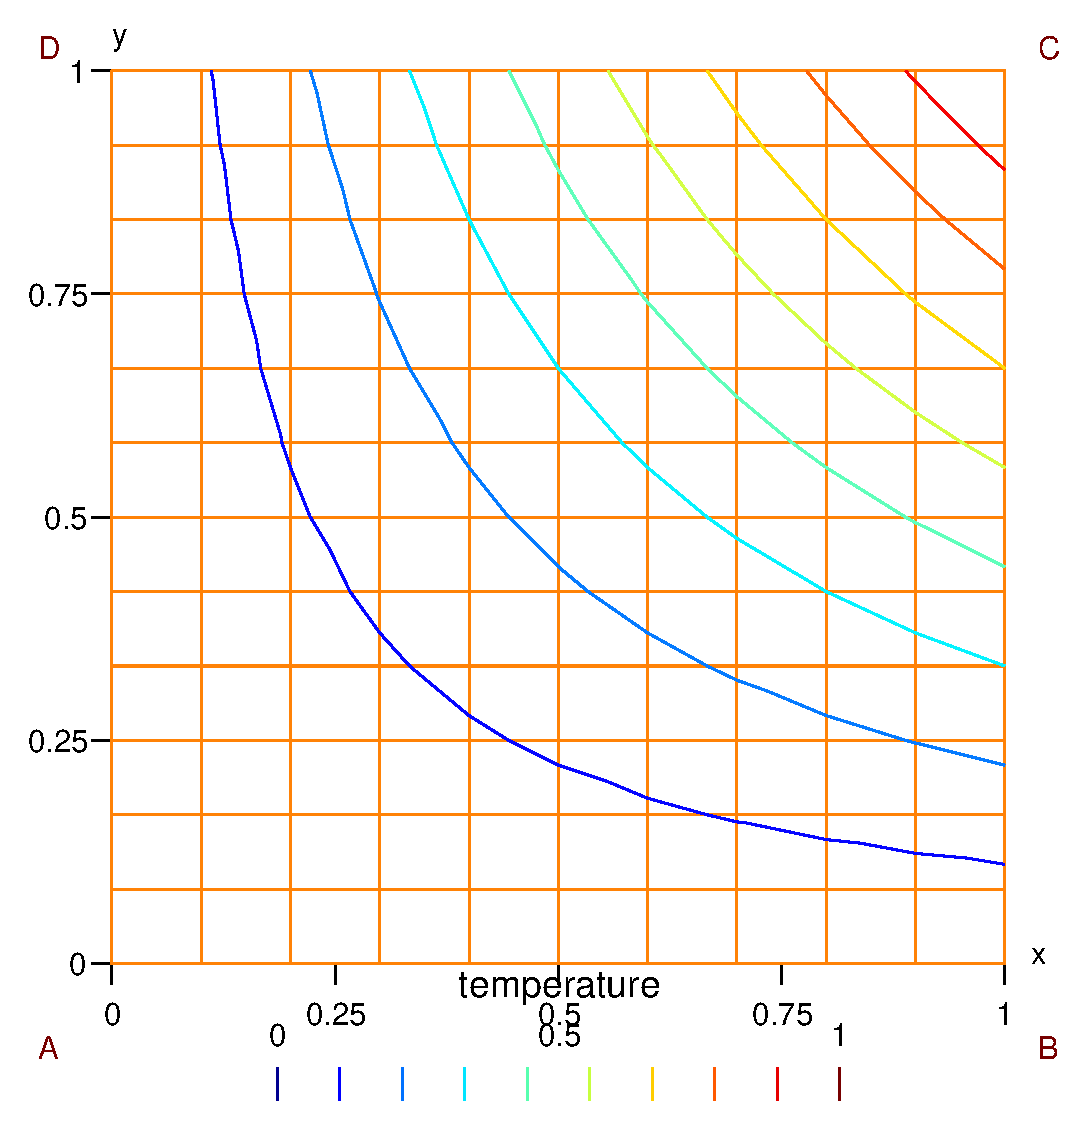
\includegraphics[width=60mm]{square-Dirichlet}
  \caption{Level lines of $u$}
  \label{\numb section 6.\numb fig 1}
\end{figure}

We stress again that the examples in this section show a rather rudimentary way of
using finite elements in \maniFEM.
We are working hard to reach a more elegant, compact and high-level style.
The user should have the possibility to declare the partial differential equation
through a compact declaration of the corresponding variational formulation.

Another limitation of {\maniFEM} is that this type of finite element is rather slow.
This is so because each docking operation implies a lot of symbolic calculations;
the same happens when we differentiate and then integrate functions.
There are three ways of circumventing this limitation.
The first one is : if your mesh is made of identical finite elements
(like the example in the present paragraph), you can compute the elementary matrix
just once and then assembly the global matrix from it.
It will surely be much faster.
A second way to speed up the code is to add the option {\small\tt -dNDEBUG} to the compilation
command in your {\small\tt Makefile} (see also paragraph \ref{\numb section 11.\numb parag 15}).

The third (and soundest) solution is a deep optimization of the {\maniFEM} library.
A different type of finite elements (or, rather, integrators) is presented in paragraphs
\ref{\numb section 6.\numb parag 9} and \ref{\numb section 6.\numb parag 10}.
These integrators perform a few symbolic calculations just once,
typically right after they are declared.
Only raw arithmetic operations are performed when the user actually requests the values
of integrals in order to assembly the matrix.


          %---------------------------%
\section{~~Neumann boundary conditions}\label{\numb section 6.\numb parag 3}
          %---------------------------%

Implementing zero Neumann boundary conditions does not imply any programming effort
(we don't have to do anything).
However, for imposing non-zero Neumann boundary conditions we need to compute one-dimensional
integrals.
We do this by declaring a 1D finite element which we then dock on each segment of the
part of the boundary where we need to integrate.

\begin{Verbatim}[commandchars=\\\{\},formatcom=\small\tt,frame=single,
   label=parag-\ref{\numb section 6.\numb parag 3}.cpp,rulecolor=\color{coment},
   baselinestretch=0.94,framesep=2mm                                            ]
   \verm{FiniteElement} \azul{fe_bdry} ( \textcolor{tag}{tag}::with_master, \textcolor{tag}{tag}::segment,
                           \textcolor{tag}{tag}::Lagrange, \textcolor{tag}{tag}::of_degree, 1 );
   \verm{Integrator} \azul{integ_bdry} = fe_bdry .set_integrator ( \textcolor{tag}{tag}::Gauss, \textcolor{tag}{tag}::seg_3 );

   \cinza{// ... assemble the matrix ...}

   \verm{Function} \azul{heat_source} = y*y;
   \cinza{// impose Neumann boundary conditions du/dn = heat_source :}
   \verm{Mesh}::Iterator \azul{it} = DA .iterator ( \textcolor{tag}{tag}::over_segments );
   for ( it .reset(); it .in_range(); it++ )
   \{  \verm{Cell} \azul{seg} = *it;
      fe_bdry .dock_on ( seg );
      \verm{Cell} \azul{V} = seg .base() .reverse();
      assert ( V .is_positive() );
      size_t \azul{i} = numbering [V];
      \verm{Function} \azul{psiV} = fe_bdry .basis_function(V);
      vector_b [i] += fe_bdry .integrate ( heat_source * psiV );
      \verm{Cell} \azul{W} = seg.tip();
      assert ( W .is_positive() );
      size_t \azul{j} = numbering [W];
      \verm{Function} \azul{psiW} = fe_bdry .basis_function(W);
      vector_b [j] += fe_bdry .integrate ( heat_source * psiW );  \}
\end{Verbatim}

One may object that there is no need for a 1D finite element, a 1D integrator should be enough.
We agree; the user should have the possibility to attach a 1D integrator to a 2D finite element.
This is object of on-going work.

Also, in this paragraph we switch to triangular finite elements (see the source code,
file {\small\tt examples-manual/parag-6.3.cpp} in the distribution tree of \maniFEM).


          %------------------------------%
\section{~~Automatic numberig of vertices}\label{\numb section 6.\numb parag 4}
          %------------------------------%

In previous examples we have built a {\small\tt map} for handling numbering of vertices.
In this paragraph we show how to use instead the automatic numbering associated to the
finite element itself.
The method {\small\tt\verm{FiniteElement}::build\_\,global\_\,numbering} creates
an object which is similar to {\small\tt std::map} but uses a different mechanism.
It modifies the process of creating new cells (vertices, in this specfic case)
by ading a new function to the list of functions
{\small\tt\verm{Cell}::init\_\,pos\_\,cell[0]},
invoked by {\small\tt\verm{Cell}::Core} constructors
(see paragraph \ref{\numb section 11.\numb parag 10}).
Space will be reserved for a {\small\tt size\_\,t} value for each new vertex, and
this value will be used for numbering vertices.

\begin{Verbatim}[commandchars=\\\{\},formatcom=\small\tt,frame=single,
   label=parag-\ref{\numb section 6.\numb parag 4}.cpp,rulecolor=\color{coment},
   baselinestretch=0.94,framesep=2mm                                            ]
   \verm{FiniteElement} \azul{fe} ( \textcolor{tag}{tag}::with_master, \textcolor{tag}{tag}::quadrangle,
                      \textcolor{tag}{tag}::Lagrange, \textcolor{tag}{tag}::of_degree, 1  );
   \verm{Cell}::Numbering & \azul{numbering} = fe .build_global_numbering ( \textcolor{tag}{tag}::vertices );
\end{Verbatim}

In this approach, the access to the index of a given vertex is very fast (constant time)
because the index is stored within the {\small\tt\verm{Cell}::Core}, so no search is needed.
In contrast, when using a {\small\tt map} as shown in paragraph
\ref{\numb section 6.\numb parag 2}, a search is necessary through all vertices of the mesh.
Due to the implementation of the {\small\tt map} class in {\tt STL}, this search takes
logarithmic time.
The only advantage of the approach described in paragraph \ref{\numb section 6.\numb parag 2}
is that the user has full contol of the numbering (see below).

Using the numbering associated to the finite element itself has the following disadvantage.
This automatic numbering process does not distinguish between vertices created at the user's
request and other vertices used internally by different components of {\maniFEM};
these vertices are invisible to the user.
As a consequence, in some cases the numbering may be not contiguous.
Lines of the global matrix corresponding to ``missing'' vertices are not significant in any way.
Columns corresponding to missing vertices are not significant either (because they will only
have zero entries).
However, the solver of the linear system will complain that the matrix is singular.

The user should check these two numbers : {\small\tt numbering} {\small\tt.size()} and
{\small\tt ABCD}  {\small\tt .number\_\,of}  {\small\tt (}
{\small\tt\textcolor{tag}{tag}::vertices}  {\small\tt )}.
If they are not equal, measures must be taken.
For instance, a non-zero value can be inserted in the diagonal of the global matrix
at places corresponding to ``missing'' vertices.
This is equivalent to imposing a Dirichlet boundary condition on those vertices.
Since we have no way of running over the missing vertices, we first fill the entire
diagonal with ones, then erase them for existing vertices.

\begin{Verbatim}[commandchars=\\\{\},formatcom=\small\tt,frame=single,
   label=parag-\ref{\numb section 6.\numb parag 4}.cpp,rulecolor=\color{coment},
   baselinestretch=0.94,framesep=2mm                                            ]
   for ( size_t \azul{i} = 0; i < size_matrix; i++ )
      matrix_A .insert ( i, i ) = 1.;
   \verm{Mesh}::Iterator \azul{it} = ABCD .iterator ( \textcolor{tag}{tag}::over_vertices );
   for ( it .reset(); it .in_range(); it++ )
   \{  \verm{Cell} \azul{P} = *it;
      size_t \azul{i} = numbering [P];
      matrix_A .coeffRef ( i, i ) = 0.;  \}
\end{Verbatim}

The rest of the code is identical to paragraph \ref{\numb section 6.\numb parag 2}.

A different way around can be used, which allows the use of a {\small\tt matrix\_\,A}
with the correct dimension (equal to the number of vertices in the mesh {\small\tt ABCD}).
We simply assign the desired value to the numbering of each vertex :

\begin{Verbatim}[commandchars=\\\{\},formatcom=\small\tt,frame=single,
   rulecolor=\color{coment},baselinestretch=0.94,framesep=2mm          ]
   \verm{Mesh}::Iterator \azul{it} = ABCD .iterator ( \textcolor{tag}{tag}::over_vertices );
   size_t \azul{counter} = 0;
   for ( it .reset(); it .in_range(); it++ )
   \{  \verm{Cell} \azul{P} = *it;
      numbering [P] = counter++;  \}
\end{Verbatim}

This solution keeps the advantage of constant accesss time to the number of a vertex.
However, the information from {\small\tt numbering} {\small\tt .size()} will be misleading
(it still takes into account the ``hidden'' vertices).
You should use instead {\small\tt ABCD} {\small\tt .number\_\,of} {\small\tt (}
{\small\tt\textcolor{tag}{tag}::vertices )}; this is the dimension you should use
when declaring your global matrix.

Note that both numbering methods (presented in paragraphs \ref{\numb section 6.\numb parag 2}
and \ref{\numb section 6.\numb parag 4}) allow for retrieving
an index of a given vertex but not the other way around.
If you need to retrieve a vertex from its index you should probably use 
a vector of {\small\tt\verm{Cell}}s.


          %-------------------------------------------------%
\section{~~Triangular Lagrange finite elements of degree two}\label{\numb section 6.\numb parag 5}
          %-------------------------------------------------%

To get a quadratic Lagrange finite element, simply choose degree two; add also a 
{\small\tt\textcolor{tag}{tag}::straight} to inform {\maniFEM} that you do not want
a curved triangle.

\begin{Verbatim}[commandchars=\\\{\},formatcom=\small\tt,frame=single,
   label=parag-\ref{\numb section 6.\numb parag 5}.cpp,rulecolor=\color{coment},
   baselinestretch=0.94,framesep=2mm                                            ]
   \verm{FiniteElement} \azul{fe2} ( \textcolor{tag}{tag}::with_master, \textcolor{tag}{tag}::triangle,
                       \textcolor{tag}{tag}::Lagrange, \textcolor{tag}{tag}::of_degree, 2, \textcolor{tag}{tag}::straight );
\end{Verbatim}

This finite element has six basis functions, associated to vertices and to sides.
Note that, although the user may imagine the finite element having nodes at the middle of
each side, the {\small\tt\verm{Cell}} on which the element is docked is still a regular triangle.
This cell has only three vertices and three sides.
This is why three of the six basis functions are associated to vertices (zero-dimensional cells)
while the other three are associated to sides (one-dimensional cells).
See also paragraph \ref{\numb section 5.\numb parag 1}.

\begin{Verbatim}[commandchars=\\\{\},formatcom=\small\tt,frame=single,
   label=parag-\ref{\numb section 6.\numb parag 5}.cpp,rulecolor=\color{coment},
   baselinestretch=0.94,framesep=2mm                                            ]
      fe2 .dock_on ( small_tri );
      \cinza{//  for loop}  
         \verm{Function} \azul{psi_V} = fe2 .basis_function ( V );   \cinza{// V is a vertex of small_tri}
         \verm{Function} \azul{psi_seg} = fe2 .basis_function ( seg );  \cinza{// seg is a side of small_tri}
\end{Verbatim}

The user must provide positive vertices {\small\tt V} but oriented (possibly negative) segments
{\small\tt seg} belonging to {\small\tt small\_\,tri} {\small\tt .boundary()}.

It is worth noticing that, although we intend to work with degree two finite elements,
the coordinate system {\small\tt\azul{xy}} is still declared with
{\small\tt\textcolor{tag}{tag}::of\_\,degree,} {\small\tt\laranja{1}}
(see the source code in file {\small\tt parag-\ref{\numb section 6.\numb parag 5}.cpp}
in the distribution tree).
This is so because we use straight triangles; if we wanted curved triangles, we should
declare {\small\tt\azul{xy}} with {\small\tt\textcolor{tag}{tag}::of\_\,degree,}
{\small\tt\laranja{2}}.
Paragraph \ref{\numb section 5.\numb parag 1} gives more details.


          %--------------------------------------------------%
\section{~~Triangular Lagrange, degree two, incremental basis}
          %--------------------------------------------------%
\label{\numb section 6.\numb parag 6}

We can add a {\small\tt\textcolor{tag}{tag}::incremental\_\,basis} :

\begin{Verbatim}[commandchars=\\\{\},formatcom=\small\tt,frame=single,
   label=parag-\ref{\numb section 6.\numb parag 6}.cpp,rulecolor=\color{coment},
   baselinestretch=0.94,framesep=2mm                                            ]
   \verm{FiniteElement} \azul{fe2} ( \textcolor{tag}{tag}::with_master, \textcolor{tag}{tag}::triangle, \textcolor{tag}{tag}::Lagrange,
                       \textcolor{tag}{tag}::of_degree, 2, \textcolor{tag}{tag}::straight, \textcolor{tag}{tag}::incremental_basis );
\end{Verbatim}

This finite element is almost identical to the one presented in paragraph
\ref{\numb section 6.\numb parag 5}.
The six basis functions are not the same, but they span the same linear function space.

The set of basis functions of this element contains the three basis functions of the
Lagrange P1 element (associated to the three vertices).
In addition, there are three basis functions associated to the three sides.

The six basis functions of this finite element take the following values

[include table]

The difference relatively to the ``usual'' finite element described in paragraph
\ref{\numb section 6.\numb parag 5} lies in the interpretation
of the coefficients when we write a function $u$ as a linear combination of basis functions.
If $ u = $ $ = \sum_{\mbox{\small\tt v}} u_{\mbox{\small\tt v}} \psi_{\mbox{\small\tt v}} +
\sum_{\mbox{\small\tt s}} u_{\mbox{\small\tt s}} \psi_{\mbox{\small\tt s}} $
({\small\tt v} being vertices, {\small\tt s} being segments), then $ u_{\mbox{\small\tt v}} =
u(\mbox{\small\tt v}) $ but $ u_{\mbox{\small\tt s}} $ is not the value of $u$ at {\small\tt m};
rather, $ u_{\mbox{\small\tt s}} = 4 u(\mbox{\small\tt m}) -2 (u(\mbox{\small\tt A}) +
u(\mbox{\small\tt B})) $ (assuming {\small\tt m} is the middle point of segment {\small\tt s}
$=$ {\small\tt AB}).
This interpretation is used when imposing the Dirichlet boundary condition in the main file
{\small\tt parag-\ref{\numb section 6.\numb parag 6}.cpp}.

This finite element is especially useful in the context of quotient manifolds.


          %---------------------------------------------------%
\section{~~Quadrangular Lagrange finite elements of degree two}
          %---------------------------------------------------%
\label{\numb section 6.\numb parag 7}

To get a bi-quadratic Lagrange finite element, simply choose degree two; add also a 
{\small\tt\textcolor{tag}{tag}::straight} to inform {\maniFEM} that you do not want
a curved quadrilateral.

\begin{Verbatim}[commandchars=\\\{\},formatcom=\small\tt,frame=single,
   label=parag-\ref{\numb section 6.\numb parag 7}.cpp,rulecolor=\color{coment},
   baselinestretch=0.94,framesep=2mm                                            ]
   \verm{FiniteElement} \azul{fe2} ( \textcolor{tag}{tag}::with_master, \textcolor{tag}{tag}::quadrangle,
                       \textcolor{tag}{tag}::Lagrange, \textcolor{tag}{tag}::of_degree, 2, \textcolor{tag}{tag}::straight );
\end{Verbatim}

This finite element has nine basis functions, associated to vertices, to sides, and to the
quadrangular cell itself :

\begin{Verbatim}[commandchars=\\\{\},formatcom=\small\tt,frame=single,
   label=parag-\ref{\numb section 6.\numb parag 7}.cpp,rulecolor=\color{coment},
   baselinestretch=0.94,framesep=2mm                                            ]
      fe2 .dock_on ( small_square );
      \cinza{//  for loop}  
         \verm{Function} \azul{psi_V} = fe2 .basis_function ( V );   \cinza{// V is a vertex of small_square}
         \verm{Function} \azul{psi_seg} = fe2 .basis_function ( seg );  \cinza{// seg is a side of small_square}
      \verm{Function} \azul{psi_central} = fe2 .basis_function ( small_square );
\end{Verbatim}

The user must provide positive vertices {\small\tt V} but oriented (possibly negative) segments
{\small\tt seg} belonging to {\small\tt small\_\,square} {\small\tt .boundary()}.
The quadrangular cell {\small\tt small\_\,square} itself may be positive or negative.

It is worth noticing that, although we intend to work with degree two finite elements,
the coordinate system {\small\tt\azul{xy}} is still declared with
{\small\tt\textcolor{tag}{tag}::of\_\,degree,} {\small\tt\laranja{1}}
(see the source code in file {\small\tt parag-\ref{\numb section 6.\numb parag 7}.cpp}
in the distribution tree).
This is so because we use straight quadrangles; if we wanted curved quadrangles, we should
declare {\small\tt\azul{xy}} with {\small\tt\textcolor{tag}{tag}::of\_\,degree,}
{\small\tt\laranja{2}}.
Paragraph \ref{\numb section 5.\numb parag 1} gives more details.


          %----------------------------------------------------%
\section{~~Quadrangular Lagrange, degree two, incremental basis}
          %----------------------------------------------------%
\label{\numb section 6.\numb parag 8}

We can add a {\small\tt\textcolor{tag}{tag}::incremental\_\,basis} :

\begin{Verbatim}[commandchars=\\\{\},formatcom=\small\tt,frame=single,
   label=parag-\ref{\numb section 6.\numb parag 8}.cpp,rulecolor=\color{coment},
   baselinestretch=0.94,framesep=2mm                                            ]
   \verm{FiniteElement} \azul{fe2} ( \textcolor{tag}{tag}::with_master, \textcolor{tag}{tag}::quadrangle, \textcolor{tag}{tag}::Lagrange,
                       \textcolor{tag}{tag}::of_degree, 2, \textcolor{tag}{tag}::straight, \textcolor{tag}{tag}::incremental_basis );
\end{Verbatim}

This finite element is almost identical to the one presented in paragraph
\ref{\numb section 6.\numb parag 7}.
The nine basis functions are not the same, but they span the same linear function space.

The set of basis functions of this element contains the four basis functions of the
Lagrange Q1 element (associated to the four vertices).
In addition, there are five basis functions associated to the four sides and to the
quadrangular cell itself.

The nine basis functions of this finite element take the following values

[include table]

The difference relatively to the ``usual'' finite element described in paragraph
\ref{\numb section 6.\numb parag 7} lies in the interpretation
of the coefficients when we write a function $u$ as a linear combination of basis functions.
If $ u = \sum_{\mbox{\small\tt v}} u_{\mbox{\small\tt v}} \psi_{\mbox{\small\tt v}} +
\sum_{\mbox{\small\tt s}} u_{\mbox{\small\tt s}} \psi_{\mbox{\small\tt s}} +
u_{\mbox{\small\tt q}} \psi_{\mbox{\small\tt q}} $
({\small\tt v} being vertices, {\small\tt s} being segments, {\small\tt q} being the quandrangular
cell itself), then $ u_{\mbox{\small\tt v}} = u(\mbox{\small\tt v}) $.
However, $ u_{\mbox{\small\tt s}} $ is not the value of $u$ at {\small\tt m};
rather, $ u_{\mbox{\small\tt s}} = u(\mbox{\small\tt m}) / 2 - ( u(\mbox{\small\tt A}) +
u(\mbox{\small\tt B}) ) / 4 $ (assuming {\small\tt m} is the middle point of segment
{\small\tt s} $=$ {\small\tt AB}).
On the other hand, $ u_{\mbox{\small\tt q}} = u(\mbox{\small\tt b}) -
\sigma_{\mbox{\small\tt s}}/2 + \sigma_{\mbox{\small\tt v}}/4 $,
where {\small\tt b} is the baricenter of cell {\small\tt q},
$ \sigma_{\mbox{\small\tt s}} $ is the sum of the values of $u$ at middle point of sides of
{\small\tt q} and $ \sigma_{\mbox{\small\tt v}} $ is the sum of the values of $u$ at vertices
of cell {\small\tt q}.
This interpretation is used when imposing the Dirichlet boundary condition in the main file
{\small\tt parag-\ref{\numb section 6.\numb parag 8}.cpp}.

This finite element is especially useful in the context of quotient manifolds.


          %--------------------------%
\section{~~Hand-coded finite elements}\label{\numb section 6.\numb parag 9}
          %--------------------------%

Paragraphs \ref{\numb section 6.\numb parag 2} -- \ref{\numb section 6.\numb parag 8}
show finite element computations where we simply take the shape functions provided by
the method {\small\tt\verm{FiniteElement}::basis\_\,function}, differentiate them
symbolically and then integrate their product through a Gauss quadrature.
This process is simple and clear from the user's viewpoint.
However, it involves a lot of symbolic computations at each docking operation and aftewards;
thus, it is quite slow.

In this paragraph we present another type of finite elements (or rather, integrators).
They are much faster at the cost of a slightly less elegant syntax.
Also, they are less flexible; finite elements described in previous paragraphs can be used
to compute integrals of very general expressions, e.g.\ {\small\tt fe} {\small\tt .integrate}
{\small\tt(} {\small\tt\verm{sin}} {\small\tt(x-y)} {\small\tt *} {\small\tt psi\_\,V.deriv(x)}
{\small\tt +} {\small\tt\verm{cos}} {\small\tt(x-y)} {\small\tt *} {\small\tt psi\_\,V.deriv(y)}%
~{\small\tt )}.
Finite elements described in this paragraph and subsequent ones only compute integrals
of certain expressions, described in paragraph \ref{\numb section 6.\numb parag 10}.
They do not keep a diffeomorphism to a master element.
The quantities relevant for finite element analysis are hard-wired in the source code
as arithmetic expressions
of the coordinates of the vertices of the cell where the finite element will later dock.

The finite element is declared by simply omitting the
{\small\tt\textcolor{tag}{tag}::with\_\,master}; the integrator gets a
{\small\tt\textcolor{tag}{tag}::hand\_\,coded}.

\begin{Verbatim}[commandchars=\\\{\},formatcom=\small\tt,frame=single,
   label=parag-\ref{\numb section 6.\numb parag 9}.cpp,rulecolor=\color{coment},
   baselinestretch=0.94,framesep=2mm                                            ]
   \verm{FiniteElement} \azul{fe} ( \textcolor{tag}{tag}::rectangle, \textcolor{tag}{tag}::Lagrange, \textcolor{tag}{tag}::of_degree, 1 );
   \verm{Integrator} \azul{integ} = fe .set_integrator ( \textcolor{tag}{tag}::hand_coded );
\end{Verbatim}

Here we use a {\small\tt\textcolor{tag}{tag}::rectangle} instead of
a {\small\tt\textcolor{tag}{tag}::quadrangle};
paragraph \ref{\numb section 6.\numb parag 10} explains why.

A hand-coded integrator requires an early declaration of the integrals we intend to compute.
One or two abstract basis functions must be declared, then the method
{\small\tt\verm{Integrator}::pre\_\,compute} is called
with a list of symbolic expressions
involving these abstract basis functions and possibly their derivatives.
Later, the user instructs the integrator to replace each of these abstract basis function
by one of the shape functions provided by the method
{\small\tt\verm{FiniteElement}::basis\_\,function}.

\begin{Verbatim}[commandchars=\\\{\},formatcom=\small\tt,frame=single,
   label=parag-\ref{\numb section 6.\numb parag 9}.cpp,rulecolor=\color{coment},
   baselinestretch=0.94,framesep=2mm                                            ]
   \verm{Function} \azul{bf1} ( \textcolor{tag}{tag}::basis_function, \textcolor{tag}{tag}::within, fe ),
            \azul{bf2} ( \textcolor{tag}{tag}::basis_function, \textcolor{tag}{tag}::within, fe );
   integ .pre_compute ( \textcolor{tag}{tag}::for_given, \textcolor{tag}{tag}::basis_functions, bf1, bf2,
                        \textcolor{tag}{tag}::integral_of, \{ bf1 .deriv(x) * bf2 .deriv(x) +
                                            bf1 .deriv(y) * bf2 .deriv(y)  \} );
\end{Verbatim}

The symbolic expressions provided to {\small\tt pre\_\,compute} must obey to rather strict
rules, described in paragraph \ref{\numb section 6.\numb parag 10}.

The {\small\tt dock\_\,on} operation has the same syntax as before :

\begin{Verbatim}[commandchars=\\\{\},formatcom=\small\tt,frame=single,
   label=parag-\ref{\numb section 6.\numb parag 9}.cpp,rulecolor=\color{coment},
   baselinestretch=0.94,framesep=2mm                                            ]
      fe .dock_on ( small_square );
\end{Verbatim}

When we call the method {\small\tt dock\_\,on}, the integrator computes all integrals
required by the user by means of {\small\tt pre\_\,compute}.
These values are kept in an internal buffer; later, when we call the method
{\small\tt integrate}, the computer simply retrieves the corresponding values from
the internal buffer.

The {\small\tt integrate} method has a syntax which is more complicated and less intuitive
than the one we have seen in paragraphs \ref{\numb section 6.\numb parag 2} --
\ref{\numb section 6.\numb parag 8}.
We do not provide an expression; this has already been done by invoking method
{\small\tt pre\_\,compute}.
We just specify the {\small\tt\textcolor{tag}{tag}::pre\_\,computed} and provide
information about which shape function should replace {\small\tt bf1} and {\small\tt bf2}
in the symbolic expressions previously declared through {\small\tt pre\_\,compute}.
If a list of several expressions has been provided to {\small\tt pre\_\,compute},
they will be retrieved all at the same time.
Thus, we must store the result in an {\small\tt std::vector} rahter than as a {\small\tt double}.
We then recover each value as components of this vector (in this example there is only
one component).

\begin{Verbatim}[commandchars=\\\{\},formatcom=\small\tt,frame=single,
   label=parag-\ref{\numb section 6.\numb parag 9}.cpp,rulecolor=\color{coment},
   baselinestretch=0.94,framesep=2mm                                            ]
         \verm{Function} \azul{psi_V} = fe.basis_function(V),
                  \azul{psi_W} = fe .basis_function (W);
         std::vector < double > \azul{result} = fe .integrate 
            ( \textcolor{tag}{tag}::pre_computed, \textcolor{tag}{tag}::replace, bf1, \textcolor{tag}{tag}::by, psi_V,
                                 \textcolor{tag}{tag}::replace, bf2, \textcolor{tag}{tag}::by, psi_W );
         assert ( result .size() ) == 1;
         matrix_A .coeffRef ( numbering[V], numbering[W] ) += result [0];
\end{Verbatim}

          %--------------------------------------%
\section{~~More details on hand-coded integrators}\label{\numb section 6.\numb parag 10}
          %--------------------------------------%

Integrators declared with {\small\tt\textcolor{tag}{tag}::hand\_\,coded} are fast at the
cost of a tedious internal implementation (relevant quantities are hard-wired in the code
as arithmetic expressions of the coordinates of the vertices of the cell where the
finite element will later be docked) and also at the cost of a slightly less elegant syntax.

They work in a three-step process which we describe below.

The first step is {\small\tt pre\_\,compute}, where the user provides a list of symbolic
expressions to be later integrated.
These expressions involve one or two abstract basis functions which have no special meaning;
they are mere place-holders for shape functions in the finite element and will be replaced
by specific shape functions after the {\small\tt dock\_\,on} operation.

The expressions listed in the last argument of {\small\tt pre\_\,compute} must obey to
rather strict rules.
They must be either linear expressions in one abstract basis function, possibly differentiated
(first order derivatives only), or bi-linear expressions in two abstract basis functions,
possibly differentiated (first order derivatives only).
In the former case, we only provide one basis function, in the latter we provide two basis
functions as arguments.
We may mix the two, including linear and bi-linear expressions in the same list;
in this case, we must provide two basis functions as arguments;
the linear expressions must depend only on the first one.

Below are some example invocations of {\small\tt pre\_\,compute} with one basis function :
\begin{Verbatim}[commandchars=\\\{\},formatcom=\small\tt,
   baselinestretch=0.94,framesep=2mm                      ]
   \verm{Function} \azul{bf} ( \textcolor{tag}{tag}::basis_function, \textcolor{tag}{tag}::within, fe );
   integ .pre_compute ( \textcolor{tag}{tag}::for_a_given, \textcolor{tag}{tag}::basis_function, bf,
                        \textcolor{tag}{tag}::integral_of, \{ bf \}                  );
   integ .pre_compute ( \textcolor{tag}{tag}::for_a_given, \textcolor{tag}{tag}::basis_function, bf,
                        \textcolor{tag}{tag}::integral_of, \{ bf .deriv(x) \}        );
   integ .pre_compute ( \textcolor{tag}{tag}::for_a_given, \textcolor{tag}{tag}::basis_function, bf,
                        \textcolor{tag}{tag}::integral_of, \{ bf .deriv(x), bf .deriv(y) \} );
   integ .pre_compute ( \textcolor{tag}{tag}::for_a_given, \textcolor{tag}{tag}::basis_function, bf,
                        \textcolor{tag}{tag}::integral_of, \{ bf .deriv(y), bf \}    );
\end{Verbatim}

Below are some example invocations of {\small\tt pre\_\,compute} with two basis functions :
\begin{Verbatim}[commandchars=\\\{\},formatcom=\small\tt,
   baselinestretch=0.94,framesep=2mm                      ]
   \verm{Function} \azul{bf1} ( \textcolor{tag}{tag}::basis_function, \textcolor{tag}{tag}::within, fe ),
            \azul{bf2} ( \textcolor{tag}{tag}::basis_function, \textcolor{tag}{tag}::within, fe );
   integ .pre_compute ( \textcolor{tag}{tag}::for_given, \textcolor{tag}{tag}::basis_functions, bf1, bf2,
                        \textcolor{tag}{tag}::integral_of, \{ bf1 * bf2 \}                );
   integ .pre_compute ( \textcolor{tag}{tag}::for_given, \textcolor{tag}{tag}::basis_functions, bf1, bf2,
                        \textcolor{tag}{tag}::integral_of, \{ bf1 * bf2, bf1 .deriv(x) * bf2 \} );

   integ .pre_compute ( \textcolor{tag}{tag}::for_given, \textcolor{tag}{tag}::basis_functions, bf1, bf2,
                        \textcolor{tag}{tag}::integral_of, \{ bf1 * bf2, bf1 .deriv(x) * bf2 .deriv(x) \} );
   integ .pre_compute ( \textcolor{tag}{tag}::for_given, \textcolor{tag}{tag}::basis_functions, bf1, bf2,
                        \textcolor{tag}{tag}::integral_of, \{ bf1 * bf2, bf1 .deriv(x) * bf2 .deriv(y) \} );
   integ .pre_compute ( \textcolor{tag}{tag}::for_given, \textcolor{tag}{tag}::basis_functions, bf1, bf2,
                        \textcolor{tag}{tag}::integral_of, \{ bf1 .deriv(x) * bf2 .deriv(x),
                                            bf1 .deriv(x) * bf2 .deriv(y),
                                            bf1 .deriv(y) * bf2 .deriv(x),
                                            bf1 .deriv(y) * bf2 .deriv(y) \} );
   integ .pre_compute ( \textcolor{tag}{tag}::for_given, \textcolor{tag}{tag}::basis_functions, bf1, bf2,
                        \textcolor{tag}{tag}::integral_of, \{ bf1 .deriv(x) * bf2 .deriv(x),
                                            bf1 * bf2, bf1 * bf2 .deriv(x) \} );
   integ .pre_compute ( \textcolor{tag}{tag}::for_given, \textcolor{tag}{tag}::basis_functions, bf1, bf2,
                        \textcolor{tag}{tag}::integral_of, \{ bf1 .deriv(x) * bf2 .deriv(x) +
                                            bf1 .deriv(y) * bf2 .deriv(y)  \} );
   integ .pre_compute ( \textcolor{tag}{tag}::for_given, \textcolor{tag}{tag}::basis_functions, bf1, bf2,
                        \textcolor{tag}{tag}::integral_of, \{ bf1, bf1 * bf2  \} );
   integ .pre_compute ( \textcolor{tag}{tag}::for_given, \textcolor{tag}{tag}::basis_functions, bf1, bf2,
                        \textcolor{tag}{tag}::integral_of, \{ bf1, bf1 .deriv(x), bf1 * bf2,
                                            bf1 .deriv(x) * bf2 .deriv(x) +
                                            bf1 .deriv(y) * bf2 .deriv(y)  \} );
\end{Verbatim}

Below are some example invocations of {\small\tt pre\_\,compute} which {\maniFEM} does not accept,
for different reasons :

\begin{Verbatim}[commandchars=\\\{\},formatcom=\small\tt,
   baselinestretch=0.94,framesep=2mm                      ]
   integ .pre_compute ( \textcolor{tag}{tag}::for_a_given, \textcolor{tag}{tag}::basis_function, bf,
      \textcolor{tag}{tag}::integral_of, \{ bf + 1. \} );  \cinza{// WRONG, symbolic expression not allowed}
   integ .pre_compute ( \textcolor{tag}{tag}::for_a_given, \textcolor{tag}{tag}::basis_function, bf,
      \textcolor{tag}{tag}::integral_of, \{ 2.* bf \} );  \cinza{// WRONG, symbolic expression not allowed}
   integ .pre_compute ( \textcolor{tag}{tag}::for_a_given, \textcolor{tag}{tag}::basis_function, bf,
      \textcolor{tag}{tag}::integral_of, \{ bf + bf .deriv(x) \} );  \cinza{// WRONG, symbolic expression not allowed}
   integ .pre_compute ( \textcolor{tag}{tag}::for_a_given, \textcolor{tag}{tag}::basis_function, bf,
      \textcolor{tag}{tag}::integral_of, \{ bf .deriv(x) + bf .deriv(y) \} );  \cinza{// WRONG, expr not allowed}
   integ .pre_compute ( \textcolor{tag}{tag}::for_given, \textcolor{tag}{tag}::basis_functions, bf1, bf2,
      \textcolor{tag}{tag}::integral_of, \{ bf2 * bf1 \} );  \cinza{// WRONG, bf1 must be first}
   integ .pre_compute ( \textcolor{tag}{tag}::for_given, \textcolor{tag}{tag}::basis_functions, bf1, bf2,
      \textcolor{tag}{tag}::integral_of, \{ bf1 - bf2 \} );  \cinza{// WRONG, symbolic expression not allowed}
   integ .pre_compute ( \textcolor{tag}{tag}::for_given, \textcolor{tag}{tag}::basis_functions, bf1, bf2,
      \textcolor{tag}{tag}::integral_of, \{ bf2, bf1 * bf2 \} );  \cinza{// WRONG, bf2 cannot appear in a linear expr}
   integ .pre_compute ( \textcolor{tag}{tag}::for_given, \textcolor{tag}{tag}::basis_functions, bf1, bf2,
      \textcolor{tag}{tag}::integral_of, \{ bf1 * bf2 * bf2 \} );  \cinza{// WRONG, symbolic expression not allowed}
\end{Verbatim}

{\ManiFEM} is under construction and many types of finite elements and integrators are
still missing.
At present, hand-coded integrators can be used in association with finite elements listed below
\begin{Verbatim}[commandchars=\\\{\},formatcom=\small\tt,
   baselinestretch=0.94,framesep=2mm                      ]
   \verm{FiniteElement} \azul{fe} ( \textcolor{tag}{tag}::triangle,   \textcolor{tag}{tag}::Lagrange, \textcolor{tag}{tag}::of_degree, 1 );
   \verm{FiniteElement} \azul{fe} ( \textcolor{tag}{tag}::quadrangle, \textcolor{tag}{tag}::Lagrange, \textcolor{tag}{tag}::of_degree, 1 );
   \verm{FiniteElement} \azul{fe} ( \textcolor{tag}{tag}::rectangle,  \textcolor{tag}{tag}::Lagrange, \textcolor{tag}{tag}::of_degree, 1 );
   \verm{FiniteElement} \azul{fe} ( \textcolor{tag}{tag}::square,     \textcolor{tag}{tag}::Lagrange, \textcolor{tag}{tag}::of_degree, 1 );
\end{Verbatim}

Note that {\small\tt\textcolor{tag}{tag}::quadrangle} and
{\small\tt\textcolor{tag}{tag}::quadrilateral} are synonymous.
However, {\small\tt\textcolor{tag}{tag}::rectangle} and {\small\tt\textcolor{tag}{tag}::square}
produce different finite elements; the integrators associated with them take advantage of
the particular geometry of the cell to perform efficient computations.
In the future, there will also be a finite element with
{\small\tt\textcolor{tag}{tag}::parallelogram}.

Another limitation is that some integrators' implementation is still incomplete and they may
reject some of the expressions listed above as correct.
For instance, in paragraph \ref{\numb section 6.\numb parag 9} we have used a finite element
declared with {\small\tt\textcolor{tag}{tag}::rectangle} which accepts the expression
{\small\tt bf1.deriv(x)} {\small\tt *} {\small\tt bf2.deriv(x)}
{\small\tt +} {\small\tt bf1.deriv(y)} {\small\tt *} {\small\tt bf2.deriv(y)}.
Had we used instead a {\small\tt\textcolor{tag}{tag}::quadrangle}, the computer would
reject this expression because the implementation of this integrator is still incomplete.
We could have achieved the same result with a slight loss in efficiency by using
{\small\tt\textcolor{tag}{tag}::quadrangle} and a vector {\small\tt\azul{result}} with two
components :

\begin{Verbatim}[commandchars=\\\{\},formatcom=\small\tt,
   baselinestretch=0.94,framesep=2mm                      ]
   \verm{FiniteElement} \azul{fe} ( \textcolor{tag}{tag}::quadrangle, \textcolor{tag}{tag}::Lagrange, \textcolor{tag}{tag}::of_degree, 1 );
   \verm{Integrator} \azul{integ} = fe .set_integrator ( \textcolor{tag}{tag}::hand_coded );

   \verm{Function} \azul{bf1} ( \textcolor{tag}{tag}::basis_function, \textcolor{tag}{tag}::within, fe ),
            \azul{bf2} ( \textcolor{tag}{tag}::basis_function, \textcolor{tag}{tag}::within, fe );
   integ .pre_compute ( \textcolor{tag}{tag}::for_given, \textcolor{tag}{tag}::basis_functions, bf1, bf2,
                        \textcolor{tag}{tag}::integral_of, \{ bf1 .deriv(x) * bf2 .deriv(x),
                                            bf1 .deriv(y) * bf2 .deriv(y) \} );

   \cinza{// run over all square cells composing ABCD}
   \verm{Mesh}::Iterator \azul{it} = ABCD .iterator ( \textcolor{tag}{tag}::over_cells_of_dim, 2 );
   for ( it .reset(); it .in_range(); it++ )
   \{  \verm{Cell} \azul{small_square} = *it;
      fe .dock_on ( small_square );

      \cinza{// run twice over the four vertices of 'small_square'}
      \verm{Mesh}::Iterator \azul{it1} = small_square .boundary() .iterator ( \textcolor{tag}{tag}::over_vertices );
      \verm{Mesh}::Iterator \azul{it2} = small_square .boundary() .iterator ( \textcolor{tag}{tag}::over_vertices );
      for ( it1 .reset(); it1 .in_range(); it1++ )
      for ( it2 .reset(); it2 .in_range(); it2++ )
      \{  \verm{Cell} \azul{V} = *it1, \azul{W} = *it2;
         \verm{Function} \azul{psi_V} = fe .basis_function(V),
                  \azul{psi_W} = fe .basis_function (W);
         std::vector < double > \azul{result} = fe .integrate 
            ( \textcolor{tag}{tag}::pre_computed, \textcolor{tag}{tag}::replace, bf1, \textcolor{tag}{tag}::by, psi_V,
                                 \textcolor{tag}{tag}::replace, bf2, \textcolor{tag}{tag}::by, psi_W );
         assert ( result .size() ) == 2;
         matrix_A .coeffRef ( numbering[V], numbering[W] ) += result [0] + result [1];
   \}  \}  \cinza{// end of for loops over vertices, end of for loop over cells}
\end{Verbatim}

A second step in using a hand-coded integrator is the {\small\tt dock\_\,on} operation.
When we call this method, the integrator receives information about the current cell
(particularly, the coordinates of the vertices)
and computes the values of the expressions (hard-wired in the source code) giving the integrals
requested by the user in the {\small\tt pre\_\,compute} step.
It computes these values for all shape functions of that finite element
(if {\small\tt pre\_\,compute} was called with one abstract basis function)
or for all pairs of shape functions (if {\small\tt pre\_\,compute} was called with two
abstract basis functions).
These values are kept in an internal buffer for later use.

The arithmetic expressions hard-wired in the source code are, in some cases, inspired
in the syntax of UFL\footnote{\small\tt https://fenics.readthedocs.io/projects/ufl/en/latest/}
and the output of FFC.\footnote{\small\tt https://fenics.readthedocs.io/projects/ffc/en/latest/}
In other cases, the expressions are bluntly and tediously computed by hand.
Method {\small\tt\verm{FiniteElement}::info()} returns a multi-line string with information
about the internal implementation of that finite element.
You may call this method just after the declaration of the element to get generic information,
or after {\small\tt pre\_\,compute} to get information specific to the expressions
listed in the last argument of {\small\tt pre\_\,compute}.
The {\small\tt info} method is only available in {\small\tt DEBUG} mode (described in paragraph
\ref{\numb section 11.\numb parag 15}).

A third step in using a hand-coded integrator is the invocation of the
{\small\tt integrate} method which simply retrieves (from the internal buffer) values 
associated with the provided shape functions.
The return value is a vector of {\small\tt double}s rather that a {\small\tt double}
in order to attend to the case when the user requests more than one expression
in the invocation of {\small\tt pre\_\,compute}.

You can use a hand-coded integrator for performing certain computations,
probably within a loop over the cells of your mesh, and then use the same integrator in another loop
to perform different computations, involving integrals of other symbolic expressions.
To achieve this, you simply call again the method {\small\tt\verm{Integrator}::pre\_\,compute}
and provide another list of quantities whose integral you will need.
You may use the same abstract basis functions, they are mere place-holders which will be replaced
by shape functions after the docking of the finite element on a cell.
